\documentclass[12pt, oneside, a4paper]{book}

%----INICIO PACKAGES----%
\usepackage[T1]{fontenc}
\usepackage[english]{babel} % linguagem do documento
\AtBeginDocument{\renewcommand{\bibname}{References}}
\usepackage[a4paper,left=3.0cm,right=3.0cm,top=2.5cm,bottom=2.5cm]{geometry} % definição das margens
\usepackage{setspace} % habilitando o espaço entre linhas
\usepackage{titlesec}
\usepackage{mathptmx}
\usepackage[utf8]{inputenc}
\usepackage[normalem]{ulem} % habilitando palavras sublinhadas
\usepackage{amssymb,amsmath,pxfonts,exscale} % permite símbolos matemáticos
\usepackage{pslatex}
\usepackage{mathrsfs} % permite uso de fontes para conjuntos
\usepackage{graphicx} % permite inserção de figuras
\usepackage[titletoc,title]{appendix}


\usepackage[export]{adjustbox}

\usepackage{algorithmic}% pacote para uso na definição do ambiente para algoritmos
\usepackage{framed}
\usepackage{booktabs}
\usepackage{comment}
\usepackage{hyperref}
\usepackage{xr}
\usepackage{color} % para colocar alguns flags de cor no texto
\usepackage[mathcal]{euler}
\usepackage{mathptmx}
\usepackage[most]{tcolorbox}
\usepackage{subfigure}
\usepackage{cite}% Mudar a referência de () para []
\usepackage[resetlabels,labeled]{multibib}
\usepackage{acronym} % acronyms
\usepackage{caption}
\usepackage{tabularx}
\usepackage{setspace}
\usepackage{float}
\usepackage{color}
\usepackage{listings}
\usepackage{amstext} % for \text macro
\usepackage{array}   % for \newcolumntype macro
\usepackage{mathtools}
\usepackage{ucs}
\usepackage{textcomp}
\usepackage{silence}
\usepackage{setspace,lipsum}
\usepackage{bookmark}
\usepackage{verbatim}
\usepackage{pdflscape}
%\usepackage{lscape}
\usepackage{rotating}
\usepackage{svg}
\usepackage{multirow}
%\usepackage{lastpage}
\usepackage{lastpage}
%\usepackage[titles]{tocloft}
\usepackage{tocbasic}
\usepackage{changepage}


\usepackage{tikz}
\usetikzlibrary{positioning, fit, backgrounds, arrows.meta}


%loutfi
\usepackage{csquotes}
\usepackage{pdfpages}


% %----- pacote nomenclaturas ----%
\usepackage{nomencl}
\makenomenclature

% 1. Remove o título e a entrada no sumário
\renewcommand{\nomname}{}

% 2. Redefine para NÃO criar \chapter* nem \section*
\makeatletter
\def\thenomenclature{%
  \nompreamble
  \list{}{%
    \labelwidth\nom@tempdim
    \leftmargin\labelwidth
    \advance\leftmargin\labelsep
    \itemsep\nomitemsep
    \let\makelabel\nomlabel}%
}
\def\endthenomenclature{%
  \endlist
  \nompostamble
}
\makeatother

% %----- pacote nomenclaturas ----%

\renewcommand{\quote}{\list{}{\rightmargin=0cm\leftmargin=4cm\topsep=0pt}\item\relax}

\newenvironment{loutfirecuo}{\begin{quoting}[rightmargin=0cm,leftmargin=1cm]\vspace{-3mm}\footnotesize\singlespacing }{\end{quoting}}

\newenvironment{loutfiquote}{\begin{quote}\begin{singlespace}\footnotesize}{\end{singlespace}\end{quote}}

%------------2019--------------------


\DeclareTOCStyleEntry[
  entrynumberformat=\entrynumberwithprefix{\textbf{\figurename}},
  dynnumwidth,
  numsep=1em
]{tocline}{figure}

\DeclareTOCStyleEntry[
  entrynumberformat=\entrynumberwithprefix{\textbf{\tablename}},
  dynnumwidth,
  numsep=1em
]{tocline}{table}

\newcommand\entrynumberwithprefix[2]{\textbf{#1\enspace #2:\hfill}}

%\DeclareTOCStyleEntry[indent=0pt]{default}{chapter}
\DeclareTOCStyleEntry[indent=0pt,entryformat=\bfseries]{tocline}{section}
\DeclareTOCStyleEntry[indent=0pt]{default}{subsection}
\DeclareTOCStyleEntry[indent=0pt]{default}{subsubsection}
\DeclareTOCStyleEntry[indent=0pt]{default}{paragraph}



% Para Tabelas
\usepackage{float}
\usepackage[normal]{threeparttable}
\usepackage[table]{colortbl}

\def\stoptable#1{%
   \hline\endtabular\par\vspace{\abovecaptionskip}%
   {\footnotesize #1}%
   \endminipage}


% Listas
\usepackage{enumitem}

\newenvironment{tight_enumerate}{
\begin{enumerate}
  \setlength{\itemsep}{0pt}
  \setlength{\parskip}{0pt}
}{\end{enumerate}}

%ABNT Cite
\usepackage[alf, 
            bibjustif, 
            abnt-etal-list=5, 
            abnt-etal-cite=2,
            abnt-emphasize=bf,
            abnt-etal-text=it,
            abnt-repeated-author-omit=no]{abntex2cite}

%------------------------------------------------------------------------------
% Arquivos Json
%------------------------------------------------------------------------------

\usepackage{xcolor}
\usepackage{listings}

\definecolor{background}{HTML}{F6F8FA}
\definecolor{delim}{RGB}{20,105,176}
\definecolor{numb}{RGB}{106,153,85}
\definecolor{string}{HTML}{C41A16}

\lstdefinelanguage{json}{
    basicstyle=\footnotesize\ttfamily,
    numbers=left,
    numberstyle=\tiny\color{gray},
    stepnumber=1,
    numbersep=8pt,
    showstringspaces=false,
    breaklines=true,
    frame=single,
    backgroundcolor=\color{background},
    morestring=[b]",
    stringstyle=\color{string},
    literate=
     *{0}{{{\color{numb}0}}}{1}
      {1}{{{\color{numb}1}}}{1}
      {2}{{{\color{numb}2}}}{1}
      {3}{{{\color{numb}3}}}{1}
      {4}{{{\color{numb}4}}}{1}
      {5}{{{\color{numb}5}}}{1}
      {6}{{{\color{numb}6}}}{1}
      {7}{{{\color{numb}7}}}{1}
      {8}{{{\color{numb}8}}}{1}
      {9}{{{\color{numb}9}}}{1}
      {:}{{{\color{delim}{:}}}}{1}
      {,}{{{\color{delim}{,}}}}{1}
      {\{}{{{\color{delim}{\{}}}}{1}
      {\}}{{{\color{delim}{\}}}}}{1}
      {[}{{{\color{delim}{[}}}}{1}
      {]}{{{\color{delim}{]}}}}{1},
}


%------------------------------------------------------------------------------
% Formatação
%------------------------------------------------------------------------------

\tolerance=1
\emergencystretch=\maxdimen
\hyphenpenalty=10000
\hbadness=10000

\linespread{1.0} % espaço entre linhas de 1.5
\setlength{\parskip}{10pt} % espaço entre parágrafos
\setcounter{secnumdepth}{4} % habilita a variável \thesubsubsection
\setcounter{tocdepth}{4} % Índice até subsubsection

\titleformat{\chapter}[hang]{\fontsize{16}{16}\normalfont\bfseries\filleft\selectfont}{\thechapter.\hspace{3pt}~}{0pt}{\normalfont\bfseries}
\titlespacing{\chapter}{0pt}{5pt}{10pt}
\titleformat{\section}[hang]{\fontsize{12}{12}\normalfont\bfseries\selectfont}{\thesection\hspace{3pt}~}{0pt}{\normalfont\bfseries}
\titlespacing{\section}{0pt}{24pt}{12pt}
\titleformat{\subsection}[hang]{\fontsize{12}{12}\normalfont\bfseries\selectfont}{\thesubsection\hspace{3pt}~}{0pt}{\normalfont\bfseries}
\titlespacing{\subsection}{0pt}{12pt}{6pt}
\titleformat{\subsubsection}[hang]{\fontsize{12}{12}\normalfont\bfseries\selectfont}{\thesubsubsection\hspace{3pt}~}{0pt}{\normalfont\bfseries}
\titlespacing{\subsubsection}{0pt}{6pt}{3pt}
\titleformat{\paragraph}[hang]{\fontsize{12}{12}\normalfont\bfseries\selectfont}{\theparagraph\hspace{3pt}~}{0pt}{\normalfont\bfseries\hspace*{3pt}}
\titlespacing{\paragraph}{0pt}{6pt}{3pt}

%------------------------------------------------------------------------------
% Chamadas Código Principal
%------------------------------------------------------------------------------

%
\makeatletter
\setlength{\@fptop}{0pt}
\makeatother
%

\newcommand{\addappendix}{%
  \section*{\appendixname}% start the appendix
  \addcontentsline{toc}{section}{\textbf{\appendixname}}% add it to the toc
  \counterwithin*{figure}{section}% optional, if you want to reset the figure counter
  \stepcounter{section}% reset counters related to section
  \renewcommand{\thesection}{\textbf{A}}% we want A
  \renewcommand{\thefigure}{\textbf{\section.\arabic{figure}}}% optional
}

\usepackage[labelfont=bf]{caption}
\counterwithout{figure}{subsubsection}
\counterwithout{figure}{subsection}
\counterwithout{figure}{section}
\counterwithout{figure}{chapter}
\counterwithout{table}{subsubsection}
\counterwithout{table}{subsection}
\counterwithout{table}{section}
\counterwithout{table}{chapter}

% Código principal onde são chamados as várias seções ou capítulos que compõem a dissertação.

\begin{document}\clearpage
    %------------------------------------------------------------------------------
% Abertura do Código para a Capa
%------------------------------------------------------------------------------
\begin{figure}[!ht]
    \centering
    
\includegraphics[scale=0.125]{FIGURAS/A_Logo_UNIRIO.pdf}
\end{figure}
\begin{center}
    UNIVERSIDADE FEDERAL DO ESTADO DO RIO DE JANEIRO \\ CENTRO DE CIÊNCIAS EXATAS E TECNOLOGIA \\ PROGRAMA DE PÓS-GRADUAÇÃO EM INFORMÁTICA
    \vskip 5.0cm

    % AGENTES DE IA NA AVALIAÇÃO CIENTÍFICA: \\
    % UMA REVISÃO AUTOMATIZADA DE PUBLICAÇÕES EM PERIÓDICOS BRASILEIROS
    INTELIGÊNCIA ARTIFICIAL NA ESCRITA CIENTÍFICA: \\
    UM TUTOR DE GÊNERO AUTOMATIZADO PARA SUBMISSÕES A CONFERÊNCIAS BRASILEIRAS

    \vskip 1.0cm

    Felipe Pereira Amaro
    \vskip 3.0cm
\end{center}
\begin{flushright}
    \textbf{Advisor}
    
    Ana Cristina Bicharra Garcia\\
    
    
	%\textbf{Co-orientador}
    
    %Dr.~Beltrano da Silva
    
\end{flushright}
\vspace{\stretch{1}} % Posiciona o próximo texto no fim da página.
\begin{center}
    RIO DE JANEIRO, RJ - BRAZIL \\ AGOSTO 2026
\end{center}
\thispagestyle{empty}

\newpage

%------------------------------------------------------------------------------
% Encerramentdo do Código para a Capa
%------------------------------------------------------------------------------
 
    %%------------------------------------------------------------------------------
% Início da folha de rosto
%------------------------------------------------------------------------------

\vspace{0.5cm}

\begin{center}
    INTELIGÊNCIA ARTIFICIAL NA ESCRITA CIENTÍFICA: \\
    UM SISTEMA MULTIAGENTE DE APOIO A SUBMISSÕES EM CONFERÊNCIAS BRASILEIRAS

    \vskip 0.5 cm

    Felipe Pereira Amaro
    \vskip 1.0 cm
\end{center}

\vspace{0.5cm}
\noindent

DISSERTATION SUBMITTED AS A PARTIAL REQUIREMENT FOR THE DEGREE OF MASTER IN INFORMATICS AT THE GRADUATE PROGRAM IN INFORMATICS OF THE FEDERAL UNIVERSITY OF THE STATE OF RIO DE JANEIRO (UNIRIO). APPROVED BY THE EXAMINING COMMITTEE BELOW.

\vskip 1.0 cm

\begin{flushleft}
    Approved By:
    \vskip 0.5 cm

\end{flushleft}

\begin{flushright}
    \rule{11.0cm}{.1mm} \\
    Ana Cristina Bicharra Garcia,~D.Sc. - UNIRIO
    \vskip 0.40 cm

    \rule{11.0cm}{.1mm}\\
    Sean Wolfgand Matsui Siqueira,~D.Sc. - UNIRIO
    \vskip 0.40 cm

    \rule{11.0cm}{.1mm}\\
    Adriana Santarosa Vivacqua,~D.Sc. - UFRJ
    \vskip 0.40 cm

    % \rule{11.0cm}{.1mm}\\
    % Henrique Prado de Sá Sousa,~D.Sc. - UNIRIO
    % \vskip 0.40 cm

    % \rule{11.0cm}{.1mm}\\
    % Juliana Baptista dos Santos França,~D.Sc. - UFRJ
    % \vskip 0.40 cm

    %\rule{11.0cm}{.1mm}\\
    %Dr.~ nome3 --- instituição
    %\vskip 0.75cm
    
%	\rule{10.0cm}{.1mm}
    
    \vskip 0.75cm
    
\end{flushright}
\vspace{\stretch{1}} % Posiciona o próximo texto no fim da página.
\begin{center}
    RIO DE JANEIRO, RJ - BRAZIL \\ SEPTEMBER 2026
\end{center}
\thispagestyle{empty}
\newpage
%------------------------------------------------------------------------------
% Fim da folha de rosto
%------------------------------------------------------------------------------
 
    %
%------------------------------------------------------------------------------
% Início da Ficha catalográfica
%------------------------------------------------------------------------------
\vspace*{14.0cm}
% Depois gerar no sistema certinho http://www.unirio.br/bibliotecacentral/fichas-catalograficas
\begin{center}
    Cataloging data prepared by the author
\end{center}
\begin{framed}
    \fontsize{10pt}{10pt}\selectfont \hspace*{0.5cm} Sobrenome, Nome e nome do meio. \\ FXXX \hspace{0.8cm} Título da Tese ou dissertação / Nome completo, ano. \\ \hspace*{1.2cm} \pageref{LastPage}p.
    \vspace{0.3cm}

    \noindent \hspace*{1.5cm} \fontsize{10pt}{10pt}\selectfont Advisor: Nome do Orientador \\ \hspace*{1.6cm}Doctoral Dissertation (caso seja tese) - Universidade Federal do Estado do Rio de Janeiro, Rio de Janeiro, Programa de Pós-Graduação em Informática, 2025.
    \vspace{0.3cm}

    \noindent \hspace*{1.7cm} \fontsize{10pt}{10pt}\selectfont 1. palavra-chave 2. palavra-chave 3. palavra-chave 4. palavra-chave 5. palavra-chave 6. palavra-chave  I. Sobrenome do Orientador, Nome e nome do meio do orientador, advisor. II. Título da tese/dissertação
    \vspace{0.3cm}
    %\begin{flushright}
        %\fontsize{10pt}{10pt}\selectfont CDD - 004.678
    %\end{flushright}
\end{framed}
\thispagestyle{empty}
\newpage
%------------------------------------------------------------------------------
% Fim da Ficha catalográfica
%------------------------------------------------------------------------------

%\begin{center}
  %\makebox[\textwidth]{\includegraphics[width=\paperwidth]{FIGURAS/ficha_catalografica.pdf}}
  %\thispagestyle{empty}
%\end{center} 
    \pagestyle{plain} 
    \pagenumbering{roman} 
    %\vspace*{\stretch{1}}
\begin{flushright}
\begin{minipage}{17em}
\textit{Dedico este trabalho a Minha Mãe, Dra Helena M da Silva Pereira, que me sempre me incentivou no mestrado e a quem eu fiz uma promessa de iniciar e concluir. Dedido também a minha esposa Luana Ferreira e minha Sogra Eva Lucia por todo apoio e colaboração  incentivo em todos os momentos que precisei me ausentar. \\Fonte}
\end{minipage}
\end{flushright}
 
    %------------------------------------------------------------------------------
% Início do Agradecimento
%------------------------------------------------------------------------------
\chapter*{\hspace*{3pt}~Agradecimentos}

\begingroup
\small

(Em construção)

\endgroup




\newpage
%------------------------------------------------------------------------------
% Fim do Agradecimento
%------------------------------------------------------------------------------
 
    % 
\chapter*{Research Itinerary}

Normalmente não usado na qualificação, só no texto final, também é opcional, e o local mais apropriado para essa seção depende de como está organizado o trabalho....

itinerário de pesquisa, opcional. itinerário de pesquisa, opcional. itinerário de pesquisa, opcional. itinerário de pesquisa, opcional. itinerário de pesquisa, opcional. itinerário de pesquisa, opcional. itinerário de pesquisa, opcional. itinerário de pesquisa, opcional. itinerário de pesquisa, opcional. itinerário de pesquisa, opcional. itinerário de pesquisa, opcional. itinerário de pesquisa, opcional. itinerário de pesquisa, opcional. itinerário de pesquisa, opcional. itinerário de pesquisa, opcional. itinerário de pesquisa, opcional. itinerário de pesquisa, opcional. itinerário de pesquisa, opcional. itinerário de pesquisa, opcional. itinerário de pesquisa, opcional. 


itinerário de pesquisa, opcional. itinerário de pesquisa, opcional. itinerário de pesquisa, opcional. itinerário de pesquisa, opcional. itinerário de pesquisa, opcional. itinerário de pesquisa, opcional. itinerário de pesquisa, opcional. itinerário de pesquisa, opcional. itinerário de pesquisa, opcional. itinerário de pesquisa, opcional. itinerário de pesquisa, opcional. itinerário de pesquisa, opcional. itinerário de pesquisa, opcional. itinerário de pesquisa, opcional. itinerário de pesquisa, opcional. itinerário de pesquisa, opcional. 

itinerário de pesquisa, opcional. itinerário de pesquisa, opcional. itinerário de pesquisa, opcional. itinerário de pesquisa, opcional. itinerário de pesquisa, opcional. itinerário de pesquisa, opcional. itinerário de pesquisa, opcional. itinerário de pesquisa, opcional. itinerário de pesquisa, opcional. itinerário de pesquisa, opcional. itinerário de pesquisa, opcional. itinerário de pesquisa, opcional. itinerário de pesquisa, opcional. itinerário de pesquisa, opcional. itinerário de pesquisa, opcional. itinerário de pesquisa, opcional. itinerário de pesquisa, opcional. itinerário de pesquisa, opcional. itinerário de pesquisa, opcional. itinerário de pesquisa, opcional. 

itinerário de pesquisa, opcional. itinerário de pesquisa, opcional. itinerário de pesquisa, opcional. itinerário de pesquisa, opcional. itinerário de pesquisa, opcional. itinerário de pesquisa, opcional. itinerário de pesquisa, opcional. itinerário de pesquisa, opcional. itinerário de pesquisa, opcional. itinerário de pesquisa, opcional. itinerário de pesquisa, opcional. itinerário de pesquisa, opcional. itinerário de pesquisa, opcional. 

\newpage 
    %------------------------------------------------------------------------------
% Início do resumo
%------------------------------------------------------------------------------
Amaro, Felipe Pereira~\textbf{Inteligência artificial na escrita científica: um tutor de gênero automatizado para submissões a conferências brasileiras}. UNIRIO, 2026. \pageref{LastPage} páginas. Qualificação de Mestrado. Programa de Pós-Graduação em Informática, UNIRIO.
\vspace{10pt}
\begin{center}
    \textbf{RESUMO}
    \vspace{10pt}
\end{center}

Este trabalho investiga o uso de modelos de linguagem de grande escala (LLMs) como instrumento de apoio à escrita científica no contexto de conferências brasileiras. O crescimento da produção científica intensificou limitações estruturais do processo de revisão por pares, como a sobrecarga de revisores, a heterogeneidade dos pareceres e a escassez de retorno estruturado a autores em início de carreira. Uma consequência particularmente onerosa para novos pesquisadores é a rejeição editorial precoce (\textit{desk rejection}): a recusa de um manuscrito antes da revisão de mérito, motivada com frequência não por falhas científicas, mas pela inadequação do texto às convenções tácitas de forma e conteúdo esperadas por uma trilha ou conferência específica. Investiga-se, para isso, o projeto de um artefato de software capaz de atuar como tutor de escrita científica. A proposta reposiciona a revisão automatizada: em vez de avaliar o manuscrito contra critérios universais de qualidade, o artefato primeiro modela o gênero comunicativo de uma trilha-alvo a partir do corpus de artigos já aceitos e então verifica a conformidade do manuscrito submetido a essa especificação, gerando diagnósticos acionáveis.
A fundamentação teórica articula a Teoria de Gêneros aplicada a Sistemas de Informação e a análise de \textit{moves} retóricos, na formulação do modelo CARS, integradas sob o método Design Science Research (DSR), envolvendo revisão de literatura, desenvolvimento do artefato e avaliação empírica por meio de estudo
de caso com pesquisadores.
Descreve-se ainda um método eficiente para analisar o conjunto de artigos de uma conferência: extração estruturada por artigo em modelo local, seguida de agregação determinística, minimizando o custo computacional.
% O Simpósio Brasileiro de Sistemas de Informação é adotado como caso de aplicação para a construção e a avaliação inicial do artefato, cuja calibração é derivada do corpus da trilha-alvo e, portanto, transferível a outras conferências mediante corpus adequado. 
Espera-se contribuir com um artefato utilizável, um conjunto de princípios de design generalizáveis e evidência empírica sobre a redução da rejeição precoce e o apoio à formação de pesquisadores no contexto brasileiro.

\textbf{Palavras-chave:}~Escrita Científica;Escrita Acadêmica; Análise de Gêneros; \textit{Moves}
Retóricos; Modelos de Linguagem de Grande Escala (LLM); Design Science Research
\newpage


% Este trabalho investiga o uso de arquiteturas multiagentes baseadas em Inteligência Artificial(IA) como instrumento de apoio à avaliação científica no contexto de periódicos brasileiros. O crescimento da produção científica intensificou limitações estruturais do processo de revisão por pares, como a sobrecarga de revisores, a heterogeneidade dos pareceres e a escassez de retorno estruturado a autores em início de carreira. Uma consequência particularmente onerosa para novos pesquisadores é a rejeição editorial precoce (desk rejection): a recusa de um manuscrito antes da revisão de mérito, motivada com frequência não por falhas científicas, mas pela inadequação do texto às convenções tácitas de forma e conteúdo esperadas por uma trilha ou conferência específica. Este trabalho investiga o projeto de um artefato de software, baseado em uma arquitetura multiagente com modelos de linguagem de grande escala (LLMs), capaz de atuar como tutor de escrita científica. A proposta reposiciona a revisão automatizada, com o objetivo de avaliar o manuscrito contra critérios universais de qualidade, o artefato primeiro modela o gênero comunicativo de uma trilha-alvo a partir do corpus de artigos já aceitos e então verifica a conformidade do manuscrito submetido a essa especificação, gerando diagnósticos acionáveis. 
% A fundamentação teórica articula a Teoria de Gêneros aplicada a Sistemas de Informação e a análise de moves retóricos, integradas sob o método Design Science Research (DSR), envolvendo revisão de literatura, desenvolvimento do artefato e avaliação empírica por meio de estudo de caso com pesquisadores.
% Descreve-se ainda um método eficiente para analisar o conjunto de artigos de uma conferência: extração estruturada por artigo em modelo local, seguida de agregação determinística, minimizando o custo computacional. Espera-se contribuir com um artefato utilizável, um conjunto de princípios de design generalizáveis e evidência empírica sobre a redução da rejeição precoce e o apoio à formação de pesquisadores no contexto brasileiro.




% \textbf{Palavras-chave:}~Revisão Científica Automatizada; Agentes de Inteligência Artificial; Teoria de Gêneros; Design Science Research; Comunicação Científica; Modelos de Linguagem de Grande Escala (LLM)
\newpage
%------------------------------------------------------------------------------
% Fim do resumo
%------------------------------------------------------------------------------
 
    %------------------------------------------------------------------------------
% Início do abstract
%------------------------------------------------------------------------------
\begin{center}
    \textbf{ABSTRACT}
    \vspace{10pt}
\end{center}

This work investigates the use of large language models (LLMs) as an instrument to support scientific writing in the context of Brazilian conferences. The growth of scientific production has intensified structural limitations of the peer review process, such as reviewer overload, heterogeneity of reviews, and scarcity of structured feedback for early-career authors. A particularly burdensome consequence for new researchers is early editorial rejection (\textit{desk rejection}): the refusal of a manuscript before merit review, frequently motivated not by scientific flaws, but by the inadequacy of the text to the tacit conventions of form and content expected by a specific track or conference. For this purpose, the design of a software artifact capable of acting as a scientific writing tutor is investigated. The proposal repositions automated review: instead of evaluating the manuscript against universal quality criteria, the artifact first models the communicative genre of a target track from the corpus of already accepted papers and then verifies the compliance of the submitted manuscript to this specification, generating actionable diagnostics.
The theoretical foundation articulates Genre Theory applied to Information Systems and the analysis of rhetorical \textit{moves}, in the formulation of the CARS model, integrated under the Design Science Research (DSR) method, involving literature review, artifact development and empirical evaluation through a case study with researchers.
An efficient method for analyzing the set of papers of a conference is also described: structured extraction per paper in a local model, followed by deterministic aggregation, minimizing computational cost.
It is expected to contribute with a usable artifact, a set of generalizable design principles and empirical evidence on the reduction of early rejection and support for the training of researchers in the Brazilian context.
\vspace{20pt}

\textbf{Keywords:}~Scientific Writing; Genre Analysis; Rhetorical \textit{Moves}; Large Language Models (LLM); Design Science Research;

%------------------------------------------------------------------------------
% Fim do abstract
%------------------------------------------------------------------------------

            
    \tableofcontents
    \listoffigures
    \listoftables
    \newpage
    \input{01_Pre_Textual/j_Indice_de_nomenclaturas}
    %\input{01_Pre_Textual/I_Indice_de_Siglas}
	
 \pagestyle{plain}% headings como argumento coloca o cabeçalho
	\pagenumbering{arabic}
    \setcounter{page}{1}
    
    %Inserir novo capíulo aqui. Um arquivo por linha
    \chapter{Introdução}\label{chap:introducao}

O crescimento exponencial da produção científica nas últimas décadas intensificou desafios estruturais do sistema de revisão por pares, como a sobrecarga de revisores, os ciclos editoriais prolongados e a variabilidade na qualidade dos pareceres. Esses fatores afetam a eficiência do processo científico e, de modo especialmente agudo, a formação de novos pesquisadores, que frequentemente enfrentam dificuldades para obter retorno estruturado e acionável sobre seus trabalhos. A revisão, quando bem conduzida, é também um espaço de aprendizado. Novos pesquisadores podem elevar a qualidade de sua produção justamente ao internalizar o que os pareceres lhes ensinam.

Paralelamente, avanços recentes em Inteligência Artificial (IA), sobretudo no desenvolvimento de modelos de linguagem de grande escala (LLMs) e de sistemas baseados em agentes, ampliaram as possibilidades de automação de tarefas cognitivas complexas. Tais tecnologias vêm sendo exploradas em diversas etapas do ciclo científico, incluindo a análise de literatura, o apoio à escrita acadêmica e a própria avaliação de manuscritos. Estudos recentes indicam que sistemas baseados em IA já são capazes de produzir avaliações com níveis de concordância comparáveis aos de revisores humanos em determinados critérios (JIN et al., 2024), sugerindo potencial para apoiar o processo editorial e reduzir o tempo de iteração entre submissões.

Este trabalho parte de um desenho de pesquisa apresentado no Simpósio Brasileiro de Sistemas de Informação (SBSI) \cite{Amaro}, que propôs uma arquitetura multiagente para apoio à avaliação científica em periódicos brasileiros. A partir das contribuições recebidas naquele fórum, o escopo é aqui aprofundado em duas direções complementares. A primeira é a mudança de propósito: de um revisor genérico para um \textbf{tutor} orientado à formação, cuja finalidade não é apenas apontar problemas, mas orientar autores em início de carreira a produzir textos adequados a um alvo editorial específico. A segunda é a introdução de \textbf{alvos} concretos de revisão: em vez de avaliar um manuscrito contra critérios universais de qualidade, o artefato passa a avaliá-lo contra o perfil de uma trilha ou conferência determinada.

\section{Contexto}

O sistema de comunicação científica brasileiro apresenta características próprias que influenciam o processo de avaliação. Veículos nacionais frequentemente operam com recursos editoriais limitados, dependem de redes restritas de revisores e enfrentam dificuldades para acompanhar o crescimento das submissões. As consequências são a demora na tramitação, a heterogeneidade dos pareceres e a escassez de \textit{feedback} estruturado aos autores. 

Esses desafios impactam de maneira significativa pesquisadores em início de carreira, que dependem do processo de revisão como espaço de aprendizado e aprimoramento metodológico. Além disso, a limitação de ferramentas automatizadas de apoio à revisão científica reduz a capacidade de editores de realizar triagens eficientes e dificulta a identificação precoce de problemas metodológicos ou lacunas na contextualização dos trabalhos.


Embora pesquisas recentes explorem o uso de LLMs na geração de retorno acadêmico, a maioria concentra-se em conferências internacionais  como ICLR Conference utilizada nos trabalhos \cite{AgentReview} e \cite{MARG} , restando pouco investigado como esses métodos podem ser adaptados às especificidades organizacionais e sociotécnicas de fóruns nacionais. 





% \begin{figure}[htb!]
% \centering
% \caption{Modern separation between the poles of nature and culture.}
% 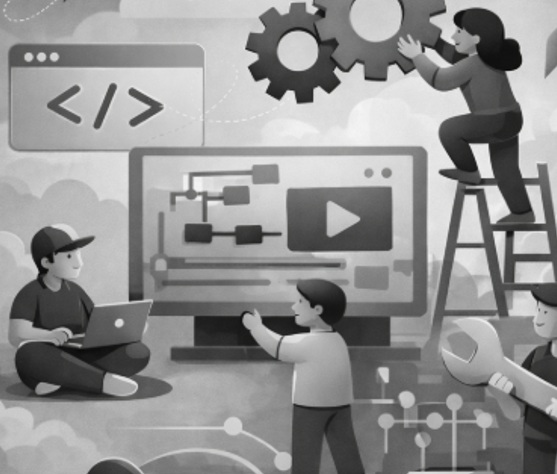
\includegraphics[width=0.8\textwidth]{FIGURAS/FIGURA_PARA_TEMPLATE.jpg}
% \caption*{\textbf{Source:} Adapted from \citeonline[p.~39]{latour2012we}}
% \label{fig:polos}
% \end{figure}





\section{Motivação}

A rejeição editorial precoce, conhecida na prática editorial como \textit{desk rejection}, é a recusa de um manuscrito antes de ser encaminhado à revisão de mérito. Uma observação central deste trabalho é que essa recusa raramente decorre de falhas científicas absolutas. Ela decorre, na maioria dos casos, da inadequação do manuscrito ao escopo, ao formato e às expectativas implícitas de uma trilha específica — em síntese, de um problema de conformidade, não de mérito. Um artigo metodologicamente sólido pode ser rejeitado na triagem simplesmente porque "não é o tipo de trabalho que aquela trilha publica".

Esse conhecimento — o que constitui um artigo bem-formado para determinada comunidade — é tácito, encontra-se distribuído nos artigos já aceitos e é adquirido lentamente, por imersão, ao longo da formação do pesquisador. É justamente o pesquisador em início de carreira quem menos o domina, e quem mais sofre suas consequências. A hipótese de trabalho que orienta esta proposta é a de que esse conhecimento tácito pode ser tornado explícito e computável a partir do corpus de artigos aceitos de uma conferência, e que um artefato pode usá-lo para orientar o autor antes da submissão.

\section{Problema e questão de pesquisa}

Identifica-se, assim, uma lacuna relacionada à compreensão de como agentes de IA podem ser estruturados para produzir avaliações contextualizadas ao gênero de uma comunidade científica, úteis à formação de novos pesquisadores. O problema de pesquisa consiste em investigar como modelar computacionalmente as convenções de gênero de uma trilha de conferência e utilizá-las para orientar autores, de modo a reduzir a rejeição editorial precoce.

Assim, o problema de pesquisa deste trabalho consiste em investigar como arquiteturas multiagentes baseadas em IA podem apoiar a avaliação sistemática de artigos científicos e contribuir para a qualificação das publicações em periódicos brasileiros.

A questão de pesquisa que orienta o estudo é:

\begin{quotation}
\noindent Agentes de IA podem contribuir para a redução da rejeição editorial a partir do corpus de artigos aceitos, e utilizá-las para produzir orientação acionável que apoie autores em início de carreira e reduza a incidência de rejeição editorial precoce?
\end{quotation}


\section{Objetivos}

O objetivo geral é projetar, construir e avaliar um artefato de software, um tutor baseado em agentes de IA que modele o gênero de uma trilha de conferência e verifique a conformidade de manuscritos a esse gênero, gerando orientação formativa. Como objetivos específicos, definem-se: 

\begin{itemize}
    \item (i) formular uma fundamentação teórica que articule a Teoria de Gêneros \cite{GenresOrgComm}, a análise de moves retóricos e a teoria de compiladores sob o método DSR
    \item (ii) especificar uma teoria de design para essa classe de artefatos, segundo a anatomia de \cite{DesignTheory}
    \item (iii) definir e implementar um método eficiente para extrair, de todo o corpus de uma conferência, a especificação de gênero de cada trilha
    \item (iv) implementar o protótipo aplicado ao SBSI e outras conferências do SOL (SBC OpenLib) \cite{solsbc}, integrando modelos locais e comerciais
    \item (v) avaliar empiricamente o artefato quanto à utilidade percebida, à validade dos diagnósticos e à concordância com avaliadores humanos.
\end{itemize}




\section{Contribuições esperadas}

Esperam-se três contribuições. 
\begin{itemize}
    \item A primeira, técnica, é o próprio artefato e o método de compilação do corpus de uma conferência em uma base de conhecimento de gênero. 

    \item A segunda, teórica, é uma teoria de design — no sentido de \cite{GenresOrgComm} %Gregor e Jones (2007) 
para artefatos de IA que apoiam a enculturação em gêneros acadêmicos, generalizável para além do SBSI. 

    \item A terceira, aplicada, é evidência empírica sobre o efeito do artefato na conformidade dos manuscritos e na percepção de utilidade por autores em formação, no contexto brasileiro.
\end{itemize}

% \section{Organização do documento}

% O Capítulo 2 apresenta a fundamentação teórica. O Capítulo 3 discute os trabalhos relacionados. O Capítulo 4 formula a solução proposta como uma teoria de design. O Capítulo 5 detalha o método de construção do artefato. O Capítulo 6 descreve o método de avaliação. O Capítulo 7 apresenta o cronograma e os resultados esperados. O Capítulo 8 traz as considerações parciais.

    

\chapter{Fundamentação Teórica}\label{chap:fundamentacao}

\section{Teoria de Gêneros de Comunicação Organizacional}
\label{sec:teoria-generos}

% A fundamentação teórica deste trabalho apoia-se na tradição que trata gêneros como ação social, na formulação desenvolvida por Yates e Orlikowski ao longo de três trabalhos complementares \cite{GenresOrgComm, GenreRepertoire, GenreSystems}.

Um gênero de comunicação organizacional é definido como uma ação comunicativa tipificada, invocada em resposta a uma situação recorrente e caracterizada por \textbf{substância} e \textbf{forma} \cite{GenresOrgComm}. Onde Uma substância diz respeito aos motivos sociais, temas e propósitos expressos na comunicação e a forma suas características e a linguísticas observável. 
Os autores identificam ao menos três aspectos da forma que são relevantes: características estruturais, como listas, campos e dispositivos de estruturação da interação; o meio de comunicação empregado; e o sistema de linguagem, incluindo grau de formalidade e vocabulário especializado.

Para exemplicificar e contextualizar o que é um gênero \cite{GenresOrgComm} utilizam o exemplo de uma reunião, que é um gênero de comunicação organizacional recorrente. A situação recorrente é a demanda organizacional por interação presencial, e a ação tipificada é a reunião em si. A substância da reunião é a execução conjunta de tarefas e responsabilidades atribuídas; sua forma inclui a marcação prévia de tempo e lugar, o meio presencial e dispositivos estruturantes como a pauta e o papel de quem preside. Uma reunião específica de um comitê de pessoal em um escritório é tratada como uma \emph{instância} do gênero, e não um gênero distinto. Uma reunião não precisa ter ata nem pauta formal para ser reconhecida como reunião, mas precisa que regras distintivas suficientes identificada, dentro daquela comunidade, como instância daquele gênero \cite{GenresOrgComm}. Porém, um encontro com pessoas conversando não necessáriamente pode ser considerada uma reunião, pois não invoca regras distintivas suficientes para ser reconhecida como instância daquele gênero.

Gêneros são encenados por meio de \textbf{regras de gênero}, que associam elementos apropriados de forma e substância a determinadas situações recorrentes \cite{GenresOrgComm}. Essas regras podem operar de maneira não explícita, operando por socialização e hábito, ou padrões explícitos destinados a regular a comunicação. Um ponto decisivo para esta pesquisa é que uma instância não precisa invocar todas as regras do gênero, mas precisa invocar regras distintivas \emph{suficientes} para que a comunidade a reconheça como instância daquele gênero. O reconhecimento é uma decisão da exclusiva da comunidade, e a ele corresponde a possibilidade de reconhecimento ou não reconhecimento.

Como gêneros existem em diferentes níveis de abstração e com diferentes escopos normativos \cite{GenresOrgComm}, é possível identificar tanto tipos amplos quanto variantes especializadas dentro de uma mesma comunidade, desde que para cada uma se possa identificar uma situação recorrente, um propósito comum e características formais compartilhadas. 
% O estudo de Devitt sobre a contabilidade fiscal, discutido pelos autores, identificou seis tipos distintos de cartas e três de memorandos praticados por uma única comunidade profissional.

Comunidades raramente dependem de um único gênero. \citeauthor{GenreRepertoire} propõem a noção de \textbf{repertório de gêneros} para designar o conjunto de gêneros rotineiramente encenados por uma comunidade, cuja composição e cujo padrão de uso revelam suas práticas comunicativas e seu processo de organização. Em comunidades acadêmicas, especificamente, a produção de conhecimento é conduzida e codificada em larga medida por meio de formas de escrita, que avaliam a informação de acordo com as normas, valores e requisitos de uma disciplina. Posteriormente,em \cite{GenreSystems} apresentam o conceito de \textbf{sistemas de gêneros}: sequências de gêneros interdependentes, encenados em uma ordem típica ou em um conjunto limitado de regras aceitáveis, cujos propósitos e formas se interligam. Um sistema de gêneros estrutura seis dimensões da interação: propósito, conteúdo, participantes, forma, tempo e lugar.

\subsection{As seis dimensões da interação e a chamada de trabalhos}
\label{sec:seis-dimensoes}
 
Ao introduzir sistema de gêneros, \cite{GenreSystems} estruturam seis dimensões da interação comunicativa: propósito, conteúdo, participantes, forma, tempo e lugar . Essas dimensões funcionam como um modelo de interação sobre o qual os membros da comunidade se apoiam, e sua utilidade analítica é dupla: ao especificar o que é esperado, o sistema de gêneros especifica também, por complemento, o que não é sancionado. Ele revela quem não está autorizado a iniciar ou receber determinados gêneros, quando e onde certos gêneros não podem ser encenados, e que conteúdo ou forma é inadequado para cada um deles.
 
Aplicadas ao fluxo editorial de um simpósio, essas dimensões oferecem uma grade de análise imediata. A observação relevante para esta pesquisa é que a chamada de trabalhos, sozinha ela opera sobre praticamente todas elas, o que a torna o gênero de maior densidade estrutural do sistema. A Tabela~\ref{tab:dimensoes-cfp} sintetiza essa análise.
 
\begin{table}[H]
\centering
\caption{As seis dimensões do sistema de gêneros e sua especificação pela chamada de trabalhos}
\label{tab:dimensoes-cfp}
\footnotesize
\begin{tabular}{|p{2.6cm}|p{4.5cm}|p{6.0cm}|}
\hline
\textbf{Dimensão} & \textbf{O que estrutura} & \textbf{Como aparece na chamada} \\
\hline
Propósito (por quê) & O propósito socialmente reconhecido do sistema e de cada gênero & Pressuposto, não enunciado: a chamada indica temas, mas não explicita o que a trilha reconhece como contribuição válida \\
Conteúdo (o quê) & Quais gêneros compõem o sistema, em que sequência, e o que cada um deve conter & Lista de tópicos de interesse, escopo da trilha e elementos esperados do manuscrito \\
Participantes (quem) & Quem inicia cada gênero e a quem ele se dirige & Definição de quem pode submeter, do papel dos revisores e da coordenação, e das restrições de anonimato \\
Forma (como) & Meio, dispositivos de estruturação e sistema de linguagem & Modelo de formatação, formato de arquivo, limite de páginas e idioma \\
Tempo (quando) & Expectativas temporais associadas a cada gênero & Cadeia de prazos de submissão, notificação e versão final \\
Lugar (onde) & Localização, física ou eletrônica, de cada gênero & Sistema de submissão para a interação assíncrona e sede do evento para a apresentação \\
\hline
\end{tabular}
\end{table}


Para exemplificar o um sistema de gêneros, \cite{GenreSystems} descrevem como uma RFP(Request for Proposal) de uma organização dá origem a uma sequência de gêneros interdependentes. O fluxo de uma RFP é comumente conhecido: uma proposta é submetida por um fornecedor, este fornecedor avalia a proposta, avalia se é capaz de aceitar a proposta e elabora um relatório com uma orçamento e suas condições, desta forma informa se aceita ou se recusa participar do leilão. Normalmente este processo envolve mais de um fornecedor que por sua vez repete executa o mesmo processo e a conclusão desta negociação é a assinatura de um contrato ou a rejeição da proposta.

Desta forma é possível observar uma semelhança entre o fluxo de uma RFP e o fluxo editorial de um simpósio científico, que envolve a submissão de artigos, a avaliação por pares e a decisão final de aceitação ou rejeição. A Tabela~\ref{tab:mapeamento-generos} apresenta o mapeamento adotado, tomando como referência o Simpósio Brasileiro de Sistemas de Informação (SBSI).

A Tabela~\ref{tab:mapeamento-generos} apresenta um mapeamento baseado nestes conceitos, tomando como referência o Simpósio Brasileiro de Sistemas de Informação (SBSI).


\begin{table}[H]
\centering
\caption{Mapeamento do fluxo editorial do SBSI às categorias da Teoria de Gêneros}
\label{tab:mapeamento-generos}
\footnotesize
\begin{tabular}{|p{4.2cm}|p{9.0cm}|}
\hline
\textbf{Elemento} & \textbf{Categoria teórica} \\
\hline
Comunidade científica de SI & Comunidade que reconhece, encena e reproduz o repertório de gêneros \\
SBSI & Sistema de gêneros institucionalizado nessa comunidade \\
SBSI 2026 & Instância do sistema de gêneros, e não um gênero distinto \\
Trilha & Recorte da situação recorrente que dá origem a um subgênero do artigo, com regras próprias \\
Chamada para submissão & Gênero iniciador do sistema; fixa participantes, forma, prazo e local \\
Submissão & Gênero respondente, análogo à proposta \\
Análise preliminar & Verificação de reconhecimento de gênero pela comunidade \\
\emph{Desk rejection} & Gênero terminal de um caminho curto do sistema \\
Revisão por pares & Gênero avaliativo, análogo ao relatório de avaliação \\
Parecer & Gênero de consolidação das avaliações em recomendação \\
Aprovação ou rejeição & Gêneros terminais mutuamente exclusivos \\
\hline
\end{tabular}
\end{table}
 
A distribuição observada na Tabela~\ref{tab:dimensoes-cfp} não é homogênea e facilmente detectável, e é esta característica que interessa a este trabalho. Cinco das seis dimensões são tratadas de maneira explícita e prescritiva na chamada, em regras de gênero verificáveis por inspeção do documento submetido. A sexta, o propósito, permanece pressuposta. \citeauthor{GenreSystems} identificam o propósito socialmente reconhecido como a característica central de identificação de um sistema de gêneros, e é precisamente por ser essencial ao pertencimento à comunidade que ele tende a permanecer implícito, transmitido por enculturação e não por enunciado.
 
Uma das consequências desta análise diz respeito à natureza dos erros que levam à rejeição. Violações nas cinco dimensões codificadas são detectáveis a partir da própria chamada, pois nela estão escritas. Violações na dimensão do propósito não são, dado que um manuscrito pode estar formatado corretamente, dentro do limite de páginas, submetido no prazo e no sistema correto, e ainda assim ser rejeitado por não realizar o tipo de contribuição que aquela trilha reconhece. 

 À luz do critério de reconhecimento formulado em \cite{GenresOrgComm}, a análise preliminar não julga primariamente o mérito da contribuição: ela verifica se o \emph{gênero respondente} submetido invocou regras distintivas suficientes para ser reconhecida como pertencente ao gênero que reivindica. Escopo incompatível, desvio de formato, falta de contribuição ou problemas metodológicos conduzem à rejeição não porque o trabalho seja ruim, mas porque ele não é reconhecida como adequada a uma instância ou subgêneros. Nesses termos, a \emph{desk rejection} é a sanção da comunidade dentro de uma instância, e frequentemente decorre de uma incompatibilidade de gênero, quando o autor escreve segundo as convenções de um gênero e submete a uma trilha, a avaliação de substância, conduzida pela revisão por pares, só ocorre depois de superado esse teste de pertencimento(Triagem de diretrizes).


\subsection{Conexão com o artefato proposto}

Esse enquadramento anterior tem uma consequência direta para o propósito do artefato desenvolvido nesta pesquisa. Dentro do que propôe a Teoria de Gêneros de Comunicação Organizacional, a dificuldade do pesquisador iniciante pode não ser necessariamente de escrita nem de método, existe a possibilidade de ainda não haver internalizado o repertório de gêneros de uma comunidade. Tal internalização ocorre por enculturação, processo tipicamente lento, tácito e dependente de exposição prolongada às práticas do grupo \cite{GenreRepertoire}. Como as regras de gênero de cada trilha não tendem a ser enunciadas de forma completa, o autor iniciante dispõe apenas de indícios parciais, distribuídos entre a chamada de trabalhos, os artigos já publicados e os pareceres que eventualmente recebe.

%CITAR ALGO RELACIONADO A DESK REJECTION.

O artefato proposto neste trabalho é conceitualmente um instrumento que acelera e tutora o autor iniciante nesta enculturação, tornando operáveis regras que de outro modo permaneceriam subentendidas. Trata-se, portanto, de uma contribuição de natureza teórica e não apenas tecnológica. Assim decorrem as três questões que orientam o desenho da solução: quais são as regras de gênero de cada trilha, como um autor pode verificar se seu manuscrito está em conformidade com elas, e de que modo um sistema multiagente pode realizar essa verificação de maneira fundamentada.

\section{Análise de \textbf{moves} retóricos}

A Teoria de Gêneros fornece o porquê sociotécnico, mas é abstrata demais para orientar diretamente a implementação. A ponte entre o construto abstrato e o texto observável é a análise de \textbf{moves} retóricos, na tradição da escrita acadêmica de \cite{GenreAnalysis}. O modelo CARS (\textbf{Create a Research Space}) decompõe a introdução de artigos científicos em movimentos retóricos recorrentes: estabelecer o território (situar a relevância e revisar a literatura), estabelecer o nicho (apontar a lacuna ou o problema) e ocupar o nicho (anunciar a contribuição e a organização do trabalho).

A importância desse modelo para a pesquisa é dupla. Primeiro, os \textbf{moves} são a manifestação observável e mensurável do gênero abstrato: onde \cite{GenresOrgComm} falam de regularidades de forma e substância, \cite{GenreAnalysis} oferece o microscópio que as torna visíveis no texto. Segundo, os \textbf{moves} são operacionalizáveis por processamento de linguagem natural, o que fornece precedente metodológico para sua extração automatizada. A articulação, portanto, é a seguinte: a Teoria de Gêneros define o construto de Sistemas de Informação; a análise de \textbf{moves} operacionaliza esse construto em unidades observáveis; 
e a extração automatizada de \textbf{moves} fornece o mecanismo pelo qual um modelo de LLM pode verificar se uma instância invocou regras distintivas suficientes para ser reconhecida como pertencente ao gênero que reivindica.

\section{Design Science Research e a anatomia da teoria de design}
%(HEVNER et al., 2004; PEFFERS et al., 2007)
O trabalho adota o método Design Science Research \cite{Hevner2004,Peffers2007}, que orienta a construção e a avaliação de artefatos como forma de produção de conhecimento. Mais do que produzir um artefato, esta pesquisa pretende produzir uma \textbf{teoria de design}, no sentido de \cite{DesignTheory}, cuja anatomia prevê oito componentes: propósito e escopo; construtos; princípios de forma e função; mutabilidade do artefato; proposições testáveis; conhecimento justificador; princípios de implementação; e instanciação expositiva. 
%Essa anatomia estrutura o Capítulo 4 e é o que permite que a contribuição transcenda o protótipo específico do SBSI, elevando-a a um conjunto de princípios generalizáveis — condição para a evolução do trabalho rumo a uma tese de doutorado.

% --- Preâmbulo (já incluídos para a Figura 1) ---
% \usepackage{tikz}
% \usetikzlibrary{positioning, fit, backgrounds, arrows.meta}

\begin{figure}[H]
  \centering
  \begin{tikzpicture}[
    >={Stealth[round]},
    font=\small,
    teoria/.style={draw, rounded corners, align=left,
                   text width=6.2cm, inner sep=8pt, minimum height=1.7cm},
    lateral/.style={draw, rounded corners, align=left, fill=gray!4,
                    text width=3.0cm, inner sep=8pt, minimum height=1.7cm},
    nivel/.style={font=\footnotesize},
    setinha/.style={->, thick, gray}
  ]

    % --- Camada 1: fenômeno ---
    \node[teoria, fill=violet!8] (t1)
      {\textbf{Teoria de Gêneros}\\[2pt]{\footnotesize Yates e Orlikowski}\\{\footnotesize \emph{fenômeno de SI}}};
    \node[lateral, right=0.7cm of t1] (l1)
      {\textbf{o quê?}\\[2pt]{\footnotesize $\rightarrow$ base de conhecimento}};

    % --- Camada 2: operacionalização ---
    \node[teoria, fill=teal!10, below=0.8cm of t1] (t2)
      {\textbf{Análise de moves --- Swales}\\[2pt]{\footnotesize modelo CARS}\\{\footnotesize \emph{operacionalização}}};
    \node[lateral, right=0.7cm of t2] (l2)
      {\textbf{como medir?}\\[2pt]{\footnotesize $\rightarrow$ extração por artigo}};

    % --- Camada 3: arquitetura (kernel) ---
    \node[teoria, fill=orange!12, below=0.8cm of t2] (t3)
      {\textbf{Teoria de compiladores}\\[2pt]{\footnotesize kernel computacional}\\{\footnotesize \emph{justificação da arquitetura}}};
    \node[lateral, right=0.7cm of t3] (l3)
      {\textbf{por que funciona?}\\[2pt]{\footnotesize $\rightarrow$ verificação e tutor}};

    % --- Setas entre as camadas ---
    \draw[setinha] (t1) -- (t2);
    \draw[setinha] (t2) -- (t3);

    % --- Moldura do DSR englobando tudo ---
    \begin{scope}[on background layer]
      \node[draw, dashed, rounded corners, fill=gray!2,
            fit=(t1)(l1)(t3)(l3), inner sep=18pt] (dsr) {};
    \end{scope}
    \node[anchor=north west, font=\bfseries]
      at ([shift={(4pt,-4pt)}]dsr.north west) {Método};

  \end{tikzpicture}
  \caption{Integração das três camadas teóricas sob o método DSR. Elaboração própria.}
  \label{fig:integracao-teorias}
\end{figure}

% > **[Figura 2 — Quadro integrador das três teorias]**
% > *Melhor local para inserção: ao final do Capítulo 2, como síntese. Diagrama em três camadas (Teoria de Gêneros → análise de moves → teoria de compiladores) dentro da moldura do DSR, cada camada associada à pergunta que responde (o quê / como medir / por que funciona) e ao estágio correspondente do artefato.*
% > 
% > Figura 2. Integração das três camadas teóricas sob o método DSR. Elaboração própria.



% ------------------------------------------------------------------------------------------------------------

% \section{Contextualization}

% Entanglement Theories seek to understand the phenomena that emerge from interactions between humans and non-humans \cite{frauenberger2019entanglement}. LAKS JJKSF JSJKSD ssk sdjfksd fsdjk dsjdks sdjkf jksjks fdjksdfj sjsjsdjfksd fsdjk dsjdks sdjkf jksjks fdjksdfj sjsjsdjfksd fsdjk dsjdks sdjkf jksjks fdjksdfj sjsjsdjfksd fsdjk dsjdks sdjkf jksjks fdjksdfj sjsjsdjfksd fsdjk dsjdks sdjkf jksjks fdjksdfj sjsjsdjfksd fsdjk dsjdks sdjkf jksjks fdjksdfj sjsjsdjfksd fsdjk dsjdks sdjkf jksjks fdjksdfj sjsj. Table \ref{tab:fontes_incerteza_tar} presents bla blab alb al.

% \begin{table}[ht!]
% \centering
% \scriptsize
% \caption{Sources of Uncertainty in ANT.}
% \rowcolors{3}{gray!10}{white}
% \begin{tabular}{p{0.19\textwidth} p{0.32\textwidth} p{0.40\textwidth}}
% \toprule
% \textbf{Soursdfsinty} & \textbf{Descsdfsdtion} & \textbf{Impliss} \\
% \midrule

% No Groxxdfsup vesdfsdfsdation: & Groups asdfdfsfsdfsdvisional assemblages. & The researcher must empiricasdfsdfsdfsdsd transformed within networks. \\

% Isolated sdfsdfsd  fsd f & sdfsd fsdf sdf sd fsddf sd sdfs fsdf dssd fs fsfsdfd sds dfsd fs. & sf sd fdf ds fds fsd sdfdsf sdf sd fsd fsd sdf sd. \\

% Human s jfsf sdfsd human Agency & sdj fskjf jkfskjfsdjksdfks jkfdsjks fjks sfkdfssfdkksskdkssdk. & sjf sdkjfsdf kjskjfsjffsfsfsdfsdfsdjkfj fkf kjs fdkfskfskfskjskjfsfsk. \\

% sd fljkfsdjk fsdjkfsdjkfsdjkfsdkjsfdkjs & s dfjksfjksfjk sdfjksd jksjksjkfskd sdk sksksksksk. & sdjkf sdjkfsfkjsdfkj sdjkfkssfkfsdkjfsdkksfksds. \\

% \bottomrule
% \end{tabular}
% \label{tab:fontes_incerteza_tar}
% \caption*{\textbf{Source:} Author's elaboration.}
% \end{table}




% The first source of uncertainty \cite[pp.~27-42]{latour2005reassembling} statkba jkdajb dakb jadjkbkadjb ajkbdajkmation, the researcher cannot simply rely on fixed categories such as ``society,'' ``organization,'' or ``users'' as starting points. It becomes necessary to observe how sfk jsfkjsd fjks fjkssfgroupings.

% The second source of uncertainty \cite[pp.~44-62]{latour2005reassembling} concerns the nature of action: action is always distributed. There is no isolated agent or clear point of origin, since ev
% This way of thinking about action profoundly transforms how we investigate social and technical phenomena. If action is always distributed, the researcher can no longer attribute it to a single agent such as a person, an institution, or a technology. Instead, it becomes necessary to trace the trajectory of the action and observe how it is produced by a network of heterogeneous elements that operate together. This requires close attention to detail: which tools were used, which norms were involved, which interpretations were mobilized, and which artifacts intervened. Agency ceases to be something that someone possesses and becomes something that occurs among many.

    \chapter{Trabalhos Relacionados}\label{chap:trabalhos_relacionados}

Este capítulo organiza os trabalhos relacionados em três frentes. A primeira reúne sistemas que usam agentes e modelos de linguagem no apoio à revisão científica. A segunda trata das bases de dados que sustentam esses sistemas e da cobertura que elas oferecem. A terceira discute limitações e riscos já documentados no uso de modelos de linguagem como avaliadores.

\section{Revisão científica assistida por agentes e LLMs}

Investigações recentes exploram o papel de agentes baseados em LLMs no processo de revisão por pares. O \textit{framework} Agent Laboratory propõe uma arquitetura de agentes capazes de conduzir diferentes fases do processo de pesquisa, incluindo revisão de literatura, planejamento experimental e redação de relatórios. Os resultados indicam que a colaboração entre humanos e agentes pode reduzir custos e acelerar o desenvolvimento científico, embora o julgamento humano permaneça essencial para garantir a qualidade das avaliações \cite{AgentLaboratory}. O foco desse trabalho, no entanto, é conduzir a pesquisa como um todo, e não avaliar a adequação de um manuscrito a um alvo editorial, que é o foco desta proposta.

Outra linha de pesquisa concentra-se na análise do próprio processo de revisão por pares. O \textit{framework} AgentReview utiliza agentes baseados em LLMs para simular interações entre autores, revisores e editores, permitindo investigar fatores sociológicos e organizacionais que influenciam decisões editoriais. Os experimentos demonstram que vieses individuais e dinâmicas de grupo podem alterar significativamente os resultados de avaliação, evidenciando a complexidade sociotécnica do processo de revisão científica \cite{AgentReview}. Essa evidência apoia uma premissa deste trabalho, a de que a decisão editorial não depende apenas do mérito absoluto do texto, mas o objetivo do AgentReview é estudar o processo, e não orientar o autor antes da submissão.

Há também esforços voltados especificamente à geração automática de pareceres científicos. O método MARG \nomenclature{MARG}{Multi-Agent Review Generation} propõe o uso de múltiplos agentes especializados que analisam diferentes aspectos do artigo, como experimentos, clareza textual e impacto científico. Estudos empíricos mostram que a abordagem multiagente produz comentários mais específicos e úteis do que sistemas baseados em um único agente, indicando vantagens da especialização e da cooperação entre agentes na tarefa de revisão \cite{MARG}. Na mesma direção, o \textit{framework} DeepReview propõe uma abordagem em múltiplos estágios que emula o processo de revisores especialistas, incorporando verificação de novidade por meio de recuperação de literatura, avaliação multidimensional e verificação de confiabilidade baseada em evidências. O modelo resultante, DeepReviewer-14B, foi treinado sobre um conjunto de dados curado com anotações estruturadas e demonstrou desempenho superior ao de sistemas maiores em tarefas de predição de notas e geração de pareceres \cite{DeepReview}.

Esta proposta aproveita duas contribuições desse conjunto de trabalhos. Da arquitetura do MARG, aproveita a ideia de agentes especializados com papéis distintos. Do DeepReview, aproveita o uso de revisões humanas reais como insumo da avaliação. A proposta se distancia deles, porém, em dois pontos. O MARG e o DeepReview avaliam o manuscrito contra critérios de qualidade tomados como universais, como solidez metodológica, novidade e contribuição, enquanto o artefato proposto avalia a adequação a um gênero específico, o de uma trilha de conferência. Além disso, a verificação de novidade do DeepReview, apoiada em recuperação de literatura, introduz um julgamento de mérito absoluto. Se esse julgamento fosse acoplado à verificação de gênero, não seria possível atribuir à modelagem de gênero o efeito observado na avaliação do artefato. Por isso ele não integra o componente avaliado nesta fase, sendo tratado como fronteira de rejeição em trabalho futuro.

\section{Bases de dados de revisão e cobertura}

Os sistemas descritos dependem de conjuntos de dados de revisões humanas em volume, e é aqui que se revela a lacuna que motiva esta pesquisa. As revisões que alimentam esses trabalhos vêm em sua maioria de conferências internacionais de aprendizado de máquina e processamento de linguagem natural, cujos pareceres são disponibilizados pela plataforma OpenReview. O conjunto PeerRead foi um dos primeiros a reunir revisões e decisões editoriais de venues como ACL, NIPS e ICLR para fins de pesquisa \cite{PeerRead2018}. Mais recentemente, o ReviewArena reuniu, em escala, revisões de sete famílias de conferências internacionais, com decisões, réplicas dos autores e o texto integral dos artigos, e constitui hoje uma das maiores bases públicas voltadas à revisão por LLMs \cite{ReviewArena}.

Apesar da escala, essas bases apresentam dois problemas para o objeto desta pesquisa. O primeiro é de idioma e domínio. Elas cobrem apenas conferências internacionais de aprendizado de máquina e processamento de linguagem natural, sem representação de Sistemas de Informação, de comunicação científica em português ou de trilhas temáticas comparáveis às de conferências brasileiras. O segundo é de cobertura da rejeição. Mesmo as bases que preservam pareceres de artigos rejeitados o fazem de modo enviesado. No PeerRead, a seção do NIPS contém revisões apenas de artigos aceitos, e os artigos do arXiv não têm revisão associada, o que limita seu uso para estudar a fronteira entre aceitação e rejeição. Vale notar ainda que a estrutura dos pareceres varia entre conferências e edições nessas bases, o que reforça, em vez de contradizer, a premissa de que o gênero do parecer é específico de cada comunidade.

Não há, até onde se levantou, conjunto público de revisões humanas de artigos científicos brasileiros que inclua artigos rejeitados. Os periódicos nacionais que adotaram avaliação aberta publicam somente pareceres de artigos aceitos, e a Sociedade Brasileira de Computação disponibiliza apenas os anais das conferências, sem os pareceres \cite{solsbc}. Essa ausência tem consequência direta para o projeto. Ela impede, por ora, fundamentar empiricamente um componente que modele a fronteira entre aceitação e rejeição no contexto brasileiro. Por isso o artefato é concebido em duas fases. A primeira modela a conformidade de gênero a partir do corpus de artigos aceitos e pode ser avaliada desde já. 
A segunda dependeria da construção de um corpus de artigos rejeitados, na ausência de um corpus de revisões brasileiras o ReviewArena viabiliza a contrução do segundo agente, pois fornece as revisões negativas reais. E como trabalho futuro, a busca por um corpus de revisões humanas de artigos científicos brasileiros.


\section{Limitações e riscos de LLMs como avaliadores}

O uso de LLMs na avaliação de manuscritos não está livre de falhas, e conhecer essas falhas orienta decisões de projeto do artefato. Li et al. \citeonline{WhereLLMWrong} propõem um \textit{framework} de perturbação multinível guiado por aspectos para diagnosticar as fraquezas de LLMs na revisão automatizada. Por meio de perturbações direcionadas a artigos, revisões e réplicas, os autores identificam vulnerabilidades recorrentes, como a classificação incorreta de falhas metodológicas como problemas de apresentação, a influência desproporcional de recomendações negativas fortes e a interpretação equivocada de críticas incorretas como avaliações rigorosas. Essas fragilidades persistem em diversos modelos amplamente utilizados, o que sustenta a decisão de restringir o artefato ao diagnóstico de conformidade e de manter o juízo final com o autor.

O risco não está apenas no modelo, mas também na forma como o usuário lida com ele. Em um estudo controlado sobre assistentes baseados em LLMs em outro domínio, o da busca de ajuda para uso de software, Khurana, Subramonyam e Chilana \citeonline{WhyandWhen} observaram que os participantes seguiam com frequência as orientações do assistente sem analisá-las, adotando respostas que continham imprecisões e atribuindo as falhas ao próprio desconhecimento, em vez de reconhecer as limitações do modelo. O contexto é diferente do da revisão científica, mas o achado se aplica ao público desta pesquisa. Autores em início de carreira, que ainda não dominam as convenções da comunidade, são justamente os mais propensos a acatar orientações incorretas sem questioná-las. Isso reforça a necessidade de o artefato explicitar o fundamento de cada diagnóstico, ou seja, a qual convenção de gênero ele se refere, para que a orientação possa ser interpretada e contestada pelo autor, e não recebida como veredito.

Em conjunto, esses estudos indicam que agentes de IA podem apoiar a produção científica, mas que sua utilidade depende de delimitar bem o que avaliam e de tornar transparente o motivo de cada apontamento. A lacuna que este trabalho aborda está na interseção de dois recortes ausentes na literatura examinada: o nível da trilha como unidade de análise, tratada como um subgênero com repertório próprio, e o contexto das conferências brasileiras, para o qual não há dados de revisão disponíveis publicamente.
    \input{02_Textual/C4_solucao_proposta}
    % 


\chapter{Método de Construção do Artefato}\label{chap:Método de Construção do Artefato}

Este capítulo detalha os princípios de implementação (PI) da teoria de design, isto é, como, em processo, o artefato é construído. A estratégia central responde a uma questão prática: como analisar, de forma eficiente, todos os artigos de uma conferência. O princípio que a orienta é o de que a LLM nunca processa o corpus inteiro de uma só vez; em vez disso, realiza uma passagem barata por artigo, e a construção do perfil da conferência torna-se um problema de agregação determinística sobre os registros resultantes.

\section{Visão geral: duas fases}
% , conforme a Figura 3. A Fase A,
O método divide-se em duas fases,A Aase A executada uma vez por conferência, é offline e de baixo custo: constrói a base de conhecimento de gênero. A Fase B, executada a cada manuscrito submetido, é a única em que o modelo comercial é acionado. Essa separação faz com que o custo de analisar uma conferência inteira seja dominado por operações locais, tornando o processamento do corpus completo economicamente viável.

\section{PI1 — Conversão estruturada}

Cada PDF é convertido em representação estruturada pelo Docling \cite{Docling}. Utilizando um conversor desenvolvido no âmbito deste trabalho, que configura o pipeline com reconhecimento óptico para português e inglês, preserva figuras e tabelas e aplica correções de artefatos de acentuação típicos de PDFs gerados em LaTeX. recurso especialmente relevante para o corpus brasileiro. Além do formato textual (Markdown), exporta-se a representação estruturada do documento (dicionário tipado em JSON), preservando a segmentação de seções e a tipagem de elementos (cabeçalhos, tabelas, figuras), da qual o estágio seguinte extrai atributos sem recorrer a expressões regulares sobre texto plano.

\section{PI2 — Extração por instância em modelo local}

Para cada artigo, produz-se um registro estruturado (JSON) validado por esquema (Pydantic). A extração combina dois tipos de atributo. Os determinísticos — estrutura de seções presentes, número de referências, de figuras, de tabelas, de páginas que são obtidos diretamente da representação estruturada. Os interpretativos, detecção dos moves CARS, classificação do tipo de contribuição (por exemplo, design science, survey, estudo de caso, experimento), presença de questão de pesquisa explícita  são delegados ao modelo local Mistral 7B \cite{mistral}, seção a seção, com saída restrita ao esquema. A padronização de cabeçalhos (mapeando variações como "Introdução", "1. Introdução" e "1 Introduction" a rótulos canônicos) assegura consistência à agregação. As referências, isoladas da seção correspondente, são convertidas em registros estruturados e enriquecidas via CrossRef e Semantic Scholar, suprindo a ausência do GROBID.

\section{PI3 — Agregação determinística}

Sobre o conjunto de registros, calculam-se as regularidades do gênero por trilha, sem LLM: distribuição dos tipos de contribuição, estrutura modal de seções, faixas típicas (medianas e quartis do número de referências e de páginas) e frequência de elementos (por exemplo, o percentual de artigos com questão de pesquisa explícita). Esse conjunto de estatísticas constitui a especificação de gênero da trilha, a "especificação da linguagem", no vocabulário da kernel de compiladores. Por ser estatística pura, é reprodutível e auditável, propriedade valiosa para a validação científica do trabalho.

\section{PI4 — Síntese e verificação pelo modelo forte}

Somente na Fase B, e em poucas chamadas, aciona-se o modelo comercial. Na revisão de um manuscrito, a especificação da trilha-alvo é injetada no contexto do modelo, que verifica a conformidade do registro do manuscrito, identifica desvios historicamente associados à rejeição precoce e gera orientações. É importante notar que, por ser a especificação de gênero um objeto estruturado e compacto, sua consulta pelo modelo dispensa, na maior parte dos casos, uma base vetorial: o perfil da trilha cabe integralmente no contexto. A recuperação semântica (RAG) é reservada a necessidades específicas, discutidas a seguir.

\section{Bases de conhecimento e o papel do RAG}

O trabalho distingue três repositórios de conhecimento, evitando um equívoco comum — o de tratar toda base de conhecimento como recuperação vetorial. O primeiro é a base teórica, um índice sobre a literatura de gêneros e escrita científica, para consulta conceitual, caso clássico de RAG \cite{RAG}. O segundo é o índice do corpus, sobre os artigos da conferência, com filtragem por metadados (trilha, seção, tipo de contribuição) oriundos do PI2, que serve ao Agente de Novidade e à recuperação de exemplares por trilha. O terceiro é a camada estruturada, as estatísticas de gênero do PI3, que não é recuperação vetorial: os padrões quantitativos de gênero são calculados por agregação determinística, não derivados por similaridade. Para a recuperação semântica dos dois primeiros, adota-se o BGE-M3 \cite{BGEM3}.

\section{PI5 e PI6 — Versionamento e orquestração}

Cada especificação de trilha é tratada como artefato versionado por edição da conferência (PI5), sustentando a mutabilidade descrita na Seção 4.6. A orquestração multiagente (PI6) mapeia os agentes da Seção 4.4 sobre os estágios do pipeline. Toda chamada a modelos de linguagem, locais ou comerciais, é intermediada por uma camada única de abstração (biblioteca litellm), o que materializa o princípio DP5: a alocação entre modelo local e comercial reduz-se a uma decisão de configuração, favorecendo a reprodutibilidade e a documentação das escolhas de design.

% > [Figura 4 — Esquema do registro estruturado por artigo]
% > Melhor local para inserção: ao final da Seção 5.3. Representação do esquema (campos determinísticos e interpretativos) que cada artigo gera, evidenciando os moves CARS e os atributos de gênero. Pode ser apresentada como figura ou como quadro; se quadro, o título vai acima.
% > 
% > Figura 4. Esquema do registro estruturado extraído por artigo. Elaboração própria.
    


\chapter{Método de Avaliação}\label{chap:avaliacao}

% Em Design Science Research, a avaliação não é etapa de verificação posterior à construção: é o que sustenta a alegação de utilidade e o que distingue a pesquisa de um relato de desenvolvimento \cite{Hevner2004}. Cabe, portanto, declarar com precisão o que este trabalho avalia e o que deixa de avaliar.

% Avalia-se a \textbf{validade interna} e a \textbf{adequação funcional} do artefato: se cada camada faz o que se propõe a fazer e se aquilo que o artefato entrega ao autor decorre do conhecimento de gênero derivado do corpus, e não do modelo de linguagem que redige o retorno. Não se avalia a utilidade percebida por autores em formação, construto perceptual que exige participantes e coleta qualitativa. Tampouco se avalia o efeito do artefato sobre taxas reais de rejeição editorial, o que exigiria acesso a manuscritos rejeitados e ao processo decisório dos comitês, ambos fora do alcance deste trabalho.

% Os procedimentos descritos a seguir são quantitativos e operam sobre evidência interna ao corpus, sendo executáveis pelo próprio pesquisador sem recrutamento de participantes.


\section{Estratégia}
\label{sec:estrategia-avaliacao}
 
A avaliação organiza-se em níveis que são correspondentes às camadas do artefato. A especificação de gênero depende da qualidade da extração, o retorno ao autor depende da adequação da especificação, de modo que cada nível só é interpretável se o anterior se sustentar. Os três empregam evidência interna ao corpus e são executáveis pelo próprio pesquisador.
 
% Este trabalho avalia a \textbf{validade interna e a adequação funcional} do artefato, e não sua utilidade em uso, cuja avaliação é remetida à etapa subsequente do trabalho pelas razões expostas na Seção~\ref{sec:utilidade-futura}.
 
\begin{table}[H]
\centering
\caption{Níveis de avaliação, construtos e procedimentos}
\label{tab:niveis-avaliacao}
\small
\begin{tabular}{|p{1.0cm}|p{3.3cm}|p{5.3cm}|p{3.7cm}|}
\hline
\textbf{Nível} & \textbf{Construto} & \textbf{Procedimento} & \textbf{Evidência} \\
\hline
1 & Validade da extração de \textbf{moves} (A2) & Comparação com anotação de referência e caracterização dos erros por \textbf{move} & Amostra anotada da trilha-alvo \\
\hline
2 & Validade da Especificação de Gênero (A3--A4) & Validação por retenção, contraste entre trilhas e sensibilidade aos limiares & Trilha-alvo e trilhas de contraste \\
\hline
3 & Contribuição da especificação ao retorno (B4) & Ablação com e sem a especificação, sobre propriedades verificáveis da saída & Artigos retidos \\
\hline
\end{tabular}
\end{table}


\section{Nível 1: validade da extração de \textbf{moves}}
\label{sec:nivel1}

Toda a cadeia repousa sobre a acurácia da rotulação. Se a extração falha de modo sistemático em um \textbf{move}, as distribuições agregadas em A3 e as regras derivadas em A4 carecem de sentido ainda que sejam computadas corretamente, e o erro se propaga sem deixar rastro nas camadas superiores.

O procedimento consiste na anotação manual de uma amostra de artigos da trilha-alvo segundo o esquema de \textbf{moves} e \textit{steps} adotado, seguida da comparação com os rótulos produzidos pelo modelo. Reportam-se precisão, revocação e medida F1 por \textbf{move}, a medida F1 macro como métrica agregada e a matriz de confusão entre categorias. A matriz importa tanto quanto os índices: confundir \textit{apontar a lacuna} com \textit{ocupar o nicho} tem consequência distinta de deixar de identificar ambos, e apenas a primeira situação preserva a frequência agregada do par.

A execução ocorre em duas etapas. Uma amostra inicial de dez artigos verifica a viabilidade do procedimento e estabiliza o protocolo de anotação, que é fixado antes de qualquer inspeção das saídas do modelo. A avaliação definitiva opera sobre amostra ampliada, estratificada de modo a não concentrar artigos de um mesmo perfil estrutural.

A anotação de referência é produzida por um único anotador, o próprio pesquisador, de modo que não se dispõe de medida de concordância entre anotadores humanos que sirva de teto interpretativo aos resultados. A alegação sustentável não é que o extrator seja acurado em termos absolutos, mas que concorda com uma anotação de referência em determinada proporção dos casos, com erros concentrados em categorias identificáveis. O produto principal do nível é a caracterização desse padrão de erro e a estimativa de seu efeito sobre as frequências agregadas.


\section{Nível 2: validade da Especificação de Gênero}
\label{sec:nivel2}

O segundo nível verifica se a especificação derivada descreve o gênero da trilha ou apenas regularidades acidentais do conjunto processado. Três procedimentos concorrem para a resposta.

\subsection*{Validação por retenção}

Parte dos artigos aceitos na trilha-alvo é separada antes da execução do Fluxo A e submetida à verificação do Fluxo B. Se a especificação captura o gênero reconhecido pela comunidade, textos que essa mesma comunidade aceitou devem satisfazer a maior parte das regras de estatuto obrigatório. Uma taxa elevada de reprovação indicaria limiares mal calibrados ou regras sem valor distintivo. A distribuição das ausências observadas entre artigos aceitos informa, ainda, a calibração do critério de suficiência enunciado em PP4: é ela que revela quantas regras um texto reconhecido pela comunidade pode deixar de invocar sem perder pertencimento.

O procedimento tem um efeito colateral que precisa ser reportado. Reter artigos reduz o corpus de derivação, e com 67 artigos na trilha-alvo uma partição de vinte por cento deixa pouco mais de cinquenta para derivar a especificação. Elementos cuja ocorrência esteja próxima de um dos cortes podem mudar de estatuto apenas em função da partição, caso em que a retenção estaria validando uma especificação distinta daquela que o artefato de fato emprega. Compara-se, por isso, a classificação obtida sobre o corpus completo com a obtida sobre o corpus reduzido, e reporta-se toda regra que migre de faixa.

\subsection*{Contraste entre trilhas}

A especificação da trilha-alvo é aplicada aos artigos das trilhas de contraste. O contraste opera em dois graus de proximidade, e é essa gradação que o torna informativo.

O primeiro grau confronta a Trilha de \textit{Pesquisa em SI} com a \textit{Main track} do ENIAC. As duas pertencem a comunidades e áreas distintas, compartilhando apenas o formato editorial da SBC, de modo que uma taxa de conformidade substancialmente inferior à dos artigos retidos indica que as regras capturam algo próprio da trilha-alvo, e não propriedades genéricas de artigos publicados em eventos da sociedade.

O segundo grau é o mais exigente e deriva especificações separadas para a \textit{Main track} e a \textit{Undergraduate track} do ENIAC, comparando-as entre si. As duas trilhas compartilham evento, chamada, período, corpo de revisores e área de conhecimento, variando apenas o subgênero. Se as especificações resultantes forem indistinguíveis, a trilha não é o nível de resolução adequado e a decisão perde sustentação. Reporta-se o conjunto de elementos cujo estatuto difere entre as duas e a magnitude dessa diferença.

\subsection*{Sensibilidade aos limiares}

O procedimento percorre a faixa plausível de valores dos dois cortes que convertem frequência em estatuto e reporta quantas e quais regras mudam de classificação, bem como o efeito de cada configuração sobre a validação por retenção. O resultado esperado não é um valor ótimo, mas a identificação de faixas de estabilidade e de pontos de ruptura. Regras que preservam seu estatuto ao longo de toda a faixa constituem o núcleo estável da especificação; regras que oscilam devem ser tratadas com reserva no retorno ao autor, e a análise indica quais são.


\section{Nível 3: contribuição da especificação ao retorno}
\label{sec:nivel3}

O terceiro nível responde a uma objeção previsível: em que medida o retorno do artefato difere daquele que se obteria pedindo a um modelo de linguagem que comentasse o manuscrito.

Realiza-se uma ablação sobre os artigos retidos, gerando o retorno em duas condições, com e sem a Especificação de Gênero disponível ao componente de composição, mantidos o mesmo modelo, a mesma instrução geral e o mesmo manuscrito. A comparação recai sobre propriedades verificáveis por contagem, e não sobre juízo de qualidade: a proporção de observações que declaram o suporte quantitativo da regra invocada; a proporção que referencia conteúdo específico do manuscrito, por oposição às que se aplicariam sem alteração a qualquer outro texto; e a incidência de redação substituta, que responde à preocupação levantada por \citeonline{WhyandWhen} quanto à incorporação acrítica de texto produzido por modelos de linguagem.

A escolha de propriedades contáveis é deliberada. Comparar as duas condições quanto à qualidade percebida exigiria avaliadores e reintroduziria, no nível destinado a isolar a contribuição da especificação, a variável que os três níveis procuram manter fora. O que se pretende estabelecer aqui não é que o retorno seja bom, mas que ele deva algo à especificação.


\section{Critérios de sucesso}
\label{sec:criterios}

Cada nível produz números, e números só decidem alguma coisa se o critério estiver fixado antes da execução. A Tabela~\ref{tab:criterios} registra os critérios adotados. Eles são decisões de projeto, e não constantes derivadas da literatura; sua função é impedir que o resultado seja interpretado depois de conhecido.

\begin{table}[H]
\centering
\caption{Critérios de sucesso por nível}
\label{tab:criterios}
\small
\begin{tabular}{|p{1.0cm}|p{5.6cm}|p{6.8cm}|}
\hline
\textbf{Nível} & \textbf{Critério} & \textbf{Interpretação de um resultado adverso} \\
\hline
1 & Medida F1 macro acima do patamar fixado, sem \textbf{move} obrigatório abaixo de um piso individual & Extração inadequada para sustentar as camadas superiores; exige revisão do esquema de rotulação ou do modelo antes de prosseguir \\
\hline
2 & Maioria dos artigos retidos satisfaz as regras obrigatórias; conformidade das trilhas de contraste inferior à dos retidos; núcleo de regras estável na faixa de limiares & Especificação sem poder discriminante, descrevendo artigos científicos em geral e não o gênero da trilha \\
\hline
3 & Condição com especificação supera a condição sem especificação nas três propriedades contadas & O retorno não deve à modelagem de gênero aquilo que entrega, e a contribuição do artefato não se distingue do uso direto de um modelo de linguagem \\
\hline
\end{tabular}
\end{table}

Os patamares numéricos do Nível~1 são fixados no protocolo de anotação, antes da execução. Registra-se que um resultado adverso em qualquer nível é achado da pesquisa, e não falha a ser contornada: estabelecer que a modelagem de gênero por derivação empírica não sustenta um tutor de conformidade seria contribuição legítima ao conhecimento, ainda que negativa.


\section{Avaliação de utilidade percebida}
\label{sec:utilidade-futura}

A utilidade percebida do Modo Tutor por autores em início de formação é construto perceptual e não admite substituto computacional: requer participantes, seus próprios manuscritos e coleta de dados qualitativos. Está prevista para a etapa subsequente do trabalho, como estudo exploratório com um pequeno número de mestrandos do programa, mediante termo de consentimento livre e esclarecido e observância dos procedimentos institucionais aplicáveis.

A postergação é escolha de escopo. Os três níveis aqui descritos estabelecem que o artefato mede o que se propõe a medir e que aquilo que ele acrescenta ao retorno decorre do conhecimento de gênero derivado do corpus. Avaliar utilidade antes dessas condições produziria percepções sobre um sistema cujos eventuais problemas não poderiam ser atribuídos a nenhuma camada em particular: um participante insatisfeito não distinguiria uma extração ruim de uma especificação mal calibrada ou de um texto mal redigido.


\section{Ameaças à validade}
\label{sec:ameacas}

\textbf{Anotador único.} A anotação de referência é produzida pelo pesquisador, o que implica ausência de medida de concordância e risco de viés na direção do comportamento esperado do extrator. Mitiga-se fixando o protocolo de anotação antes da inspeção dos resultados do modelo e reportando o padrão de erro em lugar de acurácia absoluta.

\textbf{Ausência de validação por especialistas.} A pertinência das regras não é submetida a revisores experientes da trilha, o que impede detectar regras que a comunidade reconheça e o corpus não revele. Os procedimentos do Nível~2 atestam que as regras descrevem o corpus e discriminam entre trilhas, não que sejam exaustivas.

\textbf{Viés de sobrevivência.} O corpus contém apenas artigos aceitos. A validação por retenção estabelece que a especificação é compatível com textos aprovados, não que a não conformidade implique rejeição. Nenhum resultado deste capítulo autoriza afirmação sobre a fronteira entre aceitação e recusa.

\textbf{Dependência entre níveis.} Erros sistemáticos do extrator propagam-se às camadas superiores e podem produzir resultados internamente consistentes e substantivamente equivocados. A caracterização do erro obtida no Nível~1 deve, por isso, acompanhar a leitura dos demais níveis, e não ser tratada como etapa vencida.

\textbf{Uma edição por trilha.} As especificações derivam de uma única edição de cada evento. Regularidades próprias daquela edição não se distinguem de regularidades estáveis da trilha, e o contraste entre trilhas atenua apenas parcialmente a limitação, uma vez que ambas as trilhas do ENIAC provêm da mesma edição.

\textbf{Alcance das alegações.} Os procedimentos operam sobre uma trilha-alvo, uma língua e uma comunidade. Não se sustenta alegação de generalidade a outros gêneros acadêmicos, a outras comunidades científicas ou a outros idiomas.


\section{Síntese}
\label{sec:sintese-avaliacao}

Os três níveis respondem, em ordem, a três perguntas encadeadas: se o artefato enxerga no texto o que afirma enxergar, se o que ele deriva do corpus descreve o gênero de uma trilha em particular, e se o que ele entrega ao autor decorre dessa derivação. Respondidas afirmativamente, estabelecem a validade interna necessária para que a avaliação de utilidade com autores, descrita na Seção~\ref{sec:utilidade-futura}, produza percepções atribuíveis a alguma camada do sistema. Respondidas negativamente, indicam qual camada revisar antes de prosseguir.
    % \input{02_Textual/C7_Cronograma}
    % \input{02_Textual/C8_Resultados_parciais}
    %\input{02_Textual/C3_Metodologia}
    %\input{02_Textual/C4_Cenarios}
    %\input{02_Textual/C5_Resultados}
    %\input{02_Textual/C6_Discussao}
    %\input{02_Textual/C7_Conclusao}
    % 


\chapter*{Use of GenAI Tools in the Writing Process}

Como praticamente todo mundo está usando a IA para apoiar a tese/dissertação/qualificação, isso deve estar declarado em algum lugar (ver com seu orientador(a)(e)).

The development of this dissertation was supported by Generative Artificial Intelligence (GenAI) tools, specifically the ChatGPT 5.1 model (OpenAI), employed in a controlled, transparent, and ethically responsible manner,  bla bla bla  bla bla bla  bla bla bla  bla bla bla  bla bla bla  bla bla bla  bla bla bla  bla bla bla  bla bla bla  bla bla bla  bla bla bla  bla bla bla  bla bla bla  bla bla bla  bla bla bla  bla bla bla  bla bla bla  bla bla bla  bla bla bla  bla bla bla  bla bla bla  bla bla bla  bla bla bla  bla bla bla  bla bla bla  bla bla bla  bla bla bla  bla bla bla  bla bla bla .

The use of GenAI occurred along three main fronts:

\begin{itemize}
\item \textbf{Orthographic and grammatical revision of text segments.} bla bla bla  bla bla bla  bla bla bla  bla bla bla  bla bla bla  bla bla bla  bla bla bla  bla bla bla  bla bla bla  bla bla bla  bla bla bla  bla bla bla  bla bla bla  bla bla bla  bla bla bla  bla bla bla  bla bla bla  bla bla bla  bla bla bla  bla bla bla  bla bla bla  bla bla bla  bla bla bla 

\item \textbf{Stylistic inspiration and reformulation.}  bla bla bla  bla bla bla  bla bla bla  bla bla bla  bla bla bla  bla bla bla  bla bla bla  bla bla bla  bla bla bla  bla bla bla  bla bla bla  bla bla bla  bla bla bla  bla bla bla  bla bla bla  bla bla bla  bla bla bla  bla bla bla  bla bla bla  bla bla bla  bla bla bla  bla bla bla  bla bla bla  bla bla bla  bla bla bla  bla bla bla  bla bla bla  bla bla bla  bla bla bla  bla bla bla  bla bla bla  bla bla bla  bla bla bla 

\item \textbf{Translation of the dissertation into English.}  bla bla bla  bla bla bla  bla bla bla  bla bla bla  bla bla bla  bla bla bla  bla bla bla  bla bla bla  bla bla bla  bla bla bla  bla bla bla  bla bla bla  bla bla bla  bla bla bla  bla bla bla  bla bla bla  bla bla bla  bla bla bla  bla bla bla  bla bla bla  bla bla bla  bla bla bla  bla bla bla  bla bla bla  bla bla bla  bla bla bla 

\end{itemize}

The role of AI in this research was limited to refining textual form and assisting with translation, always under the direct supervision of the researcher and subject to deliberate decision-making. This practice aligns with current guidelines issued by major Brazilian academic and research institutions such as CAPES (Brazilian Federal Agency for Support and Evaluation of Graduate Education)\footnote{CAPES: Coordenação de Aperfeiçoamento de Pessoal de Nível Superior}, CNPq (National Council for Scientific and Technological Development)\footnote{CNPq: Conselho Nacional de Desenvolvimento Científico e Tecnológico}, and SBC (Brazilian Computer Society)\footnote{SBC: Sociedade Brasileira de Computação}, as well as by international editorial committees. These bodies recognize the legitimacy of using GenAI when it is transparently reported, carefully supervised, and restricted to linguistic or stylistic support.


    \addcontentsline{toc}{chapter}{References}

\bibliographystyle{03_Pos_Textual/abntex2-alf}
\bibliography{03_Pos_Textual/referencias}

\pagebreak

    %\newpage
	%\thispagestyle{empty}
    %\mbox{}
    
    %Formatação do título dos apêndices (NÃO MEXER)
    \titleformat{\chapter}[display]
        {\normalfont\huge\bfseries\centering}{\centering\chaptertitlename\ \thechapter}{20pt}{\large}
        \titlespacing*{\chapter}{0pt}{50pt}{40pt}
    
    \appendix
    %Inserir novo apêndice aqui. Um arquivo por linha
    



\chapter{Título slf sflks dskksdfds} \label{apen:bibliometria}

\section{sec jksd fsjkfs fsjd}\label{sec:bib_metodo}

We blabla bla blalb albla blalb alalbaWe blabla bla blalb albla blalb alalbaWe blabla bla blalb albla blalb alalbaWe blabla bla blalb albla blalb alalbaWe blabla bla blalb albla blalb alalbaWe blabla bla blalb albla blalb alalbaWe blabla bla blalb albla blalb alalbaWe blabla bla blalb albla blalb alalbaWe blabla bla blalb albla blalb alalbaWe blabla bla blalb albla blalb alalbaWe blabla bla blalb albla blalb alalbaWe blabla bla blalb albla blalb alalbaWe blabla bla blalb albla blalb alalbaWe blabla bla blalb albla blalb alalbaWe blabla bla blalb albla blalb alalbaWe blabla bla blalb albla blalb alalbaWe blabla bla blalb albla blalb alalbaWe blabla bla blalb albla blalb alalba \cite{ozturk2024design}, which outlines four sequential stages for conducting bibliometric research.

We blabla bla blalb albla blalb alalbaWe blabla bla blalb albla blalb alalbaWe blabla bla blalb albla blalb alalbaWe blabla bla blalb albla blalb alalbaWe blabla bla blalb albla blalb alalbaWe blabla bla blalb albla blalb alalbaWe blabla bla blalb albla blalb alalbaWe blabla bla blalb albla blalb alalbaWe blabla bla blalb albla blalb alalbaWe blabla bla blalb albla blalb alalbaWe blabla bla blalb albla blalb alalbaWe blabla bla blalb albla blalb alalbaWe blabla bla blalb albla blalb alalbaWe blabla bla blalb albla blalb alalbaWe blabla bla blalb albla blalb alalbaWe blabla bla blalb albla blalb alalbaWe blabla bla blalb albla blalb alalbaWe blabla bla blalb albla blalb alalbaWe blabla bla blalb albla blalb alalbaWe blabla bla blalb albla blalb alalbaWe blabla bla blalb albla blalb alalba


\subsection{sub sub ssubus bus bsu}

We blabla bla blalb albla blalb alalbaWe blabla bla blalb albla blalb alalbaWe blabla bla blalb albla blalb alalbaWe blabla bla blalb albla blalb alalbaWe blabla bla blalb albla blalb alalbaWe blabla bla blalb albla blalb alalbaWe blabla bla blalb albla blalb alalbaWe blabla bla blalb albla blalb alalbaWe blabla bla blalb albla blalb alalbaWe blabla bla blalb albla blalb alalbaWe blabla bla blalb albla blalb alalbaWe blabla bla blalb albla blalb alalbaWe blabla bla blalb albla blalb alalbaWe blabla bla blalb albla blalb alalbaWe blabla bla blalb albla blalb alalbaWe blabla bla blalb albla blalb alalbaWe blabla bla blalb albla blalb alalbaWe blabla bla blalb albla blalb alalbaWe blabla bla blalb albla blalb alalbaWe blabla bla blalb albla blalb alalbaWe blabla bla blalb albla blalb alalbaWe blabla bla blalb albla blalb alalbaWe blabla bla blalb albla blalb alalbaWe blabla bla blalb albla blalb alalbaWe blabla bla blalb albla blalb alalbaWe blabla bla blalb albla blalb alalbaWe blabla bla blalb albla blalb alalbaWe blabla bla blalb albla blalb alalbaWe blabla bla blalb albla blalb alalbaWe blabla bla blalb albla blalb alalbaWe blabla bla blalb albla blalb alalbaWe blabla bla blalb albla blalb alalbaWe blabla bla blalb albla blalb alalbaWe blabla bla blalb albla blalb alalbaWe blabla bla blalb albla blalb alalbaWe blabla bla blalb albla blalb alalbaWe blabla bla blalb albla blalb alalbaWe blabla bla blalb albla blalb alalbaWe blabla bla blalb albla blalb alalbaWe blabla bla blalb albla blalb alalbaWe blabla bla blalb albla blalb alalba

blab alb alblab alb alblab alb alblab alb alblab alb alblab alb alblab alb alblab alb alblab alb alblab alb alblab alb alblab alb alblab alb alblab alb alblab alb alblab alb alblab alb alblab alb alblab alb alblab alb alblab alb alblab alb alblab alb alblab alb alblab alb alblab alb alblab alb alblab alb al

\begin{figure}[htb!]
\centering
\caption{Base Search String}
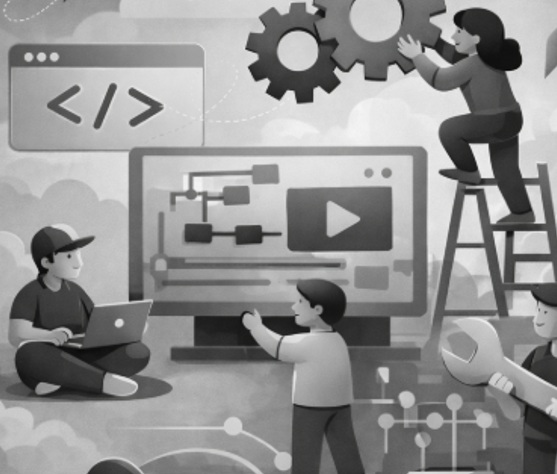
\includegraphics[width=0.8\textwidth]{FIGURAS/FIGURA_PARA_TEMPLATE.jpg}
\caption*{\textbf{Source:} Author’s elaboration.}
\label{fig:string_APENDICE}
\end{figure}

    % 

\chapter{R Script for blabjkak dblab albalab}\label{apen:script}

blalba bla ba (Figure \ref{fig:r_code_appendix}) blab alb albl alba lbalb albla blab alb albl alba lbalb albla blab alb albl alba lbalb albla blab alb albl alba lbalb albla blab alb albl alba lbalb albla blab alb albl alba lbalb albla blab alb albl alba lbalb albla blab alb albl alba lbalb albla blab alb albl alba lbalb albla blab alb albl alba lbalb albla blab alb albl alba lbalb albla blab alb albl alba lbalb albla blab alb albl alba lbalb albla blab alb albl alba lbalb albla blab alb albl alba lbalb albla blab alb albl alba lbalb albla blab alb albl alba lbalb albla blab alb albl alba lbalb albla blab alb albl alba lbalb albla blab alb albl alba lbalb albla blab alb albl alba lbalb albla blab alb albl alba lbalb albla blab alb albl alba lbalb albla

\begin{figure}[htb!]
\centering
\caption{R Code for Data blabl alba lbalbal}
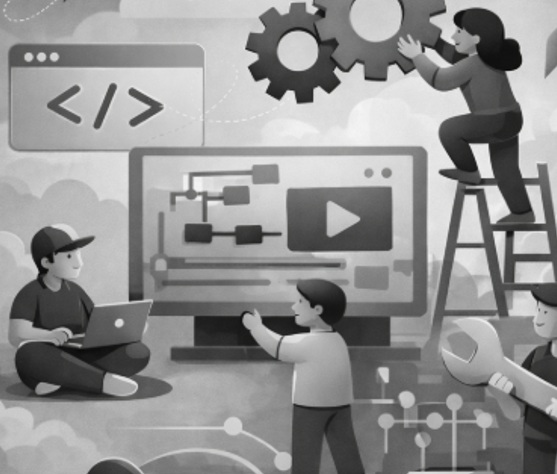
\includegraphics[width=0.7\textwidth]{FIGURAS/FIGURA_PARA_TEMPLATE.jpg}
\caption*{\textbf{Source:} Author’s elaboration.}
\label{fig:r_code_appendix}
\end{figure}

    
\end{document}